\documentclass{beamer}
\usetheme{Madrid}

\usepackage{algorithm2e}

\title{Primality Testing}
\subtitle{With Algorithm Implementations in Python}
\author{Jackson Howe - Supervisor: Kumar}
\institute{Western University}
\date{\today}

\begin{document}

\begin{frame}
\titlepage
\end{frame}

\begin{frame}
\frametitle{Outline}
\tableofcontents
\end{frame}

\section{Introduction}


% \begin{frame}
% \frametitle{Why Should we Care About Prime Factorization?}
% \begin{itemize}
%     \item While it is relatively easy to find primes, it is very hard to factor large numbers into primes
%     \item Modern encryption algorithms exploit the fact that we can easily take two large prime numbers and multiply them together
%     \item For example, while it might be easy to factor 123,228,940 into 2, 2, 5, 23, 79, and 3391, it is hard to factor 3,695,568,429 into 2089, 1381, 61, 7, and 3
% \end{itemize}
% \end{frame}
\subsection{A History of Primality Testing}

\begin{frame}
\frametitle{A History of Primality Testing Before Computers}
\begin{itemize}
    \item \textbf{3rd century BCE} Sieve of Eratosthenes: returns all numbers less than n that are prime
    \item \textbf{1228} Fibonacci gives algorithm to determine if n is prime by dividing it by numbers up to $\sqrt{n}$
    \item \textbf{1548 - 1626} Perfect Numbers: if $2^n - 1$ is prime, then n is prime and ($2^n - 1$)($2^n - 1$) is perfect.
\end{itemize}
\end{frame}

\subsection{Why Primes are Useful}

\begin{frame}
\frametitle{Why Primes are Useful}
\begin{itemize}
    \item Primes are used in everyday life, but the main use of primes is in cryptography
    \item Cryptograpic protocols are used in web server requests, ecommerce, secure communication and data exchange, and generally enforcing privacy
\end{itemize}
    
\end{frame}

\begin{frame}
\frametitle{Why Primes are Useful}
    \begin{figure}
        \centering
        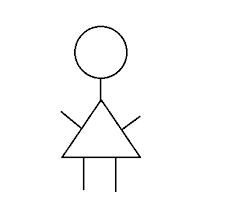
\includegraphics[width=5cm, height=5cm]{alice.png}
        
\includegraphics[width=4cm, height=5cm]{bob.png}
    \end{figure}
    \begin{itemize}
        \item Alice wants to send a message, m to Bob
        \item Bob will generate two keys, a public key and a private key
    \end{itemize}
\end{frame}

\begin{frame}{RSA}
    \begin{itemize}
        \item \textbf{Key Generation}
        \begin{itemize}
            \item N = pq, where p, q are "large" primes
            \item $\phi(N)$ = $\{a \in \mathbb{N}: 1 \leq a \leq N, \ (a, N)
            = 1\}$
            \item Choose e such that (e, $\phi(N)$) = 1
            \item public key: [N, e], private key: d $\equiv$ $e^{-1} \pmod {\phi(N)}$ 
        \end{itemize}
        \item m := unencoded message, c := cipher text
        \item \textbf{Encryption}
        \begin{itemize}
            \item c = $m^e \pmod N$
        \end{itemize}
        \item \textbf{Decryption}
        \begin{itemize}
            \item m $\equiv c^d \pmod N$
            \item $c^d \equiv m^{ed} \equiv m \pmod N$
        \end{itemize}
        \item \textbf{Finding Primes}
        \begin{itemize}
            \item \textit{Prime Number Theorem}: For numbers n $\in \mathbb{N}$ with the "same" number of digits, it will take approximately \textbf{log(n)} tries to find a prime
        \end{itemize}
    \end{itemize}
\end{frame}

\subsection{Naive Tests}

\begin{frame}
\frametitle{Naive Tests}
\begin{itemize}
    \item We search for a deterministic polynomial time with respect to the input length, so a test with complexity of the form $log^tn$, where $t \in \mathbb{N}$
\end{itemize}
\begin{block}{Primality Testing Strategy}
    For some n $\in \mathbb{N}$, $\forall$ 2 $\leq$ m $\leq$ $\sqrt{n}$, test if m $\vert$ n
\end{block}
\begin{alertblock}{Complexity}
    Complexity is O($2^{log_2(\sqrt{n})}$) + memory issues
\end{alertblock}

\end{frame}

% \begin{frame}[fragile]
% \frametitle{Sieve of Eratosthenes}

% \begin{algorithm2e}
%     \SetAlgoLined
%     \KwData{n $\in$ $\mathbb{N}$}
%     \KwResult{n in PRIMES}
    
%     A $\leftarrow$ array of Boolean values all set to True \\
%     A[0] $\leftarrow$ False \\
%     A[1] $\leftarrow$ False \\
    
%     \For {i in 1,2,...,\sqrt{n}} {
%         \If {A[i] is True} {
%             \For {j = i^2, i^2 + i, i^2 + 2i, ... \  until \ n} {
%                 A[j] $\leftarrow$ False
%             }
%         }
%     }
%     return all i such that A[i] is True
% \end{algorithm2e}
% \end{frame}

% \begin{frame}{Sieve of Eratosthenes}
%     \begin{alertblock}{Complexity}
%         $O(n\log \log n)$ + memory issues
%     \end{alertblock}
% \end{frame}

\section{Fermat's Test}

\subsection{Fermat's Test and Proof}

\begin{frame}
\frametitle{Fermat's Test}
\begin{theorem}[Fermat's Little Theorem]
    Let p be a prime number and let a $\in$ $\mathbb{Z}$ be coprime. Then 
    
    \begin{align*}
        a^{p-1} \equiv 1 \pmod p
    \end{align*}
    % \begin{equation*}
    %     $a^{p-1}$ $\equiv$  \begin{cases}
    %                 1 \ (mod \ p) \quad &\text{if} \  \, p\nmid a \\
    %                 0 \ (mod \ p) \quad &\text{if}  \ \, p \ \vert \  a \\
    %             \end{cases}
    % \end{equation*}
\end{theorem}

\begin{block}{Fermat's Test}
    for some n $\in \mathbb{N}$, 
    \begin{align*}
        \text{ if } n \nmid a \text{ and } a^{n-1} \equiv 1 \pmod n 
    \end{align*}
    then n is prime
\end{block}
% \begin{proof}
%     Idea when p $\nmid$ a involves showing that multiplying a list of a, 2a, 3a, ..., (p - 1)a returns the same result (mod p) as multiplying 1, 2, ..., (p - 1). Thus $a^{p-1}$ \cdot \ (p-1)! \  $\equiv$ (p - 1)! (mod p).
% \end{proof}
\end{frame}

\begin{frame}
\frametitle{Fermat Witnesses and Liars}
    \begin{definition}
        If \textit{a} $\in$ $\mathbb{N}$ is such that (a, n) = 1 and $a^{n-1}$ $\not\equiv$ 1 (mod n), \textit{a} is called a \textit{Fermat witness} for n and n is definitely composite
    \end{definition}
    \begin{definition}
        if \textit{a} $\in$ $\mathbb{N}$ is such that (a, n) = 1 and $a^{n-1}$ $\equiv$ 1 (mod n), but \textit{n} is composite, \textit{a} is called a \textit{Fermat liar} for n 
    \end{definition}
\end{frame}

\begin{frame}
\frametitle{Carmichael Numbers}
    \begin{itemize}
        \item Consider the number 561
        \item $2^{560}$ $\equiv$ 1 (mod 561), $5^{560}$ $\equiv$ 1 (mod 561), ..., $379^{560}$ $\equiv$ 1 (mod 561)
        \item But 561 = 3 $\cdot$ 11 $\cdot$ 17 
    \end{itemize}
    \begin{definition}
        if some number \textit{c} $\in$ $\mathbb{N}$ satisfies $a^{c-1}$ $\equiv$ 1 (mod c) for 2 $\leq$ a $\leq$ c - 1 such that (a, c) = 1, but c is composite, then \textit{c} is called a \textit{Carmichael Number}
    \end{definition}
    \begin{alertblock}{Validity}
        There are infinitely many Carmichael Numbers!
    \end{alertblock}
\end{frame}

\begin{frame}
\frametitle{Fermat's Algorithm and Probability}

\begin{algorithm2e}

    \SetAlgoLined
    \KwData{n $\in$ $\mathbb{N}$}
    \KwResult{n in PRIMES}
    
    Choose a random 2 \leq  a \leq n - 1 \\
    \If {(n, a) == 1} { \\
        \lIf {$a^{n-1}$ $\not\equiv$ 1 \pmod n} {return \  false}
        \lElse {return true}
    }
\end{algorithm2e}
\begin{block}{Primality Testing Strategy}
    For n $\in \mathbb{N}$, such that n is not a Carmichael number one Fermat test has a probability of being correct of at least 1/2. 
\end{block}
\end{frame}

\subsection{Fermat Witnesses, Liars, and Carmichael Numbers}

\section{Miller-Rabin Test}

\subsection{Miller-Rabin Algorithm}

\begin{frame}
\frametitle{Non-trivial Square Roots}
\begin{definition}
    a \textbf{non-trivial square root modulo n} is some number a not equal to 1 or n - 1 such that $a^2 \equiv 1 \pmod n$
\end{definition}

\begin{example}
    For example, 
    \begin{align*}
        4^2 \equiv 1 \pmod {15} \text{, }
    \end{align*}
    so 4 is a non-trivial square root modulo 15
\end{example}

\end{frame}

\begin{frame}
    
\frametitle{Non-trivial Square Roots}

\begin{theorem}
    For \textit{n} $\in$ $\mathbb{N}$, if n is prime, then the $x^2 \equiv 1 \pmod n$ has no nontrivial solutions (only 1 and -1)
\end{theorem}
\begin{theorem}
    For n $\in \mathbb{N}$ such that n = pq, where p and q are distinct odd primes, then $x^2 \equiv 1 \pmod n$ has non-trivial solutions
\end{theorem}
\begin{block}{Remark}
    This congruence is "stronger" than Fermat's test, as there is somewhat of a converse
\end{block}
% \begin{proof}
%     ($\rightarrow$) We prove a weaker claim in which n is the product of at least 2 distinct odd primes, call them p and q. Since (p, q) = 1, we get the system of congruences:
%     \begin{equation*}
%         \begin{aligned}
%             & x $\equiv$ 1 (mod p) \\
%             \quad & x $\equiv$ -1 (mod q)
%         \end{aligned}
%     \end{equation*}
%     By the Chinese Remainder Theorem, x = 1$\cdot$q$\cdot$$q^{-1}$ + (-1)$\cdot$p$\cdot$$p^{-1}$ (mod n) is a solution. Supposing this is trivial, we get a contradiction.
%     \\
%     ($\leftarrow$) Note that x $\equiv$ -1 (mod n) and x $\equiv$ 1 (mod n) are trivial solutions. We can see that any x that satisfies our hypotheses is congruent to one of these mod n. 
% \end{proof}
\end{frame}

\begin{frame}
\frametitle{Miller-Rabin Test}

\begin{block}{Recall}
    Fermat's Theorem:
    \begin{align*}
        a^{p-1} \equiv 1 \pmod p \text{ if } p \nmid a
    \end{align*}
    or 
    \begin{align*}
        a^{p-1} - 1 \equiv 0 \pmod p \text{ if } p \nmid a
    \end{align*}
\end{block}
\begin{block}{Difference of Squares}
    As long as $p - 1$ is even, we can continue to factor this equation as a difference of squares, we get:
    \begin{align*}
        (a^{(p-1)/2^k} - 1)(...)(a^{(p-1)/2} + 1) \equiv 0 \pmod p
    \end{align*}
\end{block}

\end{frame}

\begin{frame}

\frametitle{Miller-Rabin Test}
    \begin{algorithm2e}
        \SetAlgoLined
        \KwData{n $\in$ $\mathbb{N}$}
        \KwResult{n in PRIMES}
        
        \If {n $>$ 2 and n is even} {return false} 
        s $\leftarrow$ 0 \\
        t $\leftarrow$ n - 1 \\
        \While {t is even} {
            s $\leftarrow$ s + 1 \\
            t $\leftarrow$ t // 2 \\
            }
    \end{algorithm2e}
\end{frame}
\begin{frame}
\frametitle{Miller-Rabin Test Continued and Probability}
    \begin{algorithm2e}
        Randomly select some x $\in$ {1,2,...,n - 1} \\
        \If {x^{n-1} \not\equiv 1} {return false}
        \For {i in 1,2,...,s} {
            \If {$x^{2^it} \equiv 1\pmod n$ and $x^{2^{i-1}t} \not\equiv \pm 1 \pmod n$} {
                return false
            }
        }
        return true
    \end{algorithm2e}
    \begin{block}{Primality Testing Strategy}
        The probability this test is correct is 3/4 \textbf{always}
    \end{block}
    \begin{block}{Time Complexity}
        The time complexity is $log^3n$
    \end{block}
\end{frame}

\section{AKS Test}

\begin{frame}
\frametitle{AKS Test}
\begin{itemize}
    \item In 2002 Agrawal, Kayal, and Saxena developed a deterministic polynomial-time primality test, meaning the probability of correctness is 1
    \item The basis of the test is the fact that for X $\in$ P[x], a $\in$ $\mathbb{Z}$, n $\in$ $\mathbb{N}$, n is prime if and only if 
    \begin{align*}
        (X + a)^n \equiv X^n + a \pmod n
    \end{align*}
    \item The time complexity for this algorithm is approx. O($log^{15/2}n$), meaning that for the time being, the Miller-Rabin test is still superior for most practical applications
\end{itemize}
\end{frame}

\begin{frame}{References}
    \begin{itemize}
        \item \textit{An Introduction to Mathematical Cryptography} - Hoffstein, Pipher, Silverman
        \item \textit{An Introduction to the Theory of Numbers} - Niven, Zuckerman, Montgomery
        \item \textit{Elementary Number Theory: Primes Congruences, and Secrets} - Stein
        \item \textit{PRIMES is in P} - Agrawal, Kayal, Saxena
        \item \textit{The Miller-Rabin Randomized Primality Test} - Kleinberg, Cornell University
    \end{itemize}
\end{frame}
    
\end{document}